\section{Indgangsvælger}
\begin{frame}{Indgangsvælger - Krav}
\scriptsize{
\begin{table}[h]
\centering
\begin{tabular}{l|r}
\hline\hline
Område & Krav \\
\hline\hline
Antal trin i & 4 \\
indgangsvælgeren & \\[4pt]
Indgangsimpedans & \> 22 k\ohm \\[4pt]
Frekvensgang & \< 0,375 dB ved 20 Hz - 20 kHz, ref. 1 kHz \\
& \< 0,75 dB fra 20 Hz til 63 Hz \\
& \< 0,75 dB fra 12,5 kHz til 20 kHz \\[4pt]
Dæmpning af slukket & \> 50 dB ved 1 kHz \\
indgangssignal & \\
\hline\hline
\end{tabular}
\label{tab:krav_indgangsvaelger}
\end{table}
}
\end{frame}

\begin{frame}{Indgangsvælger - Opbygning}

\begin{figure}[h]
\centering
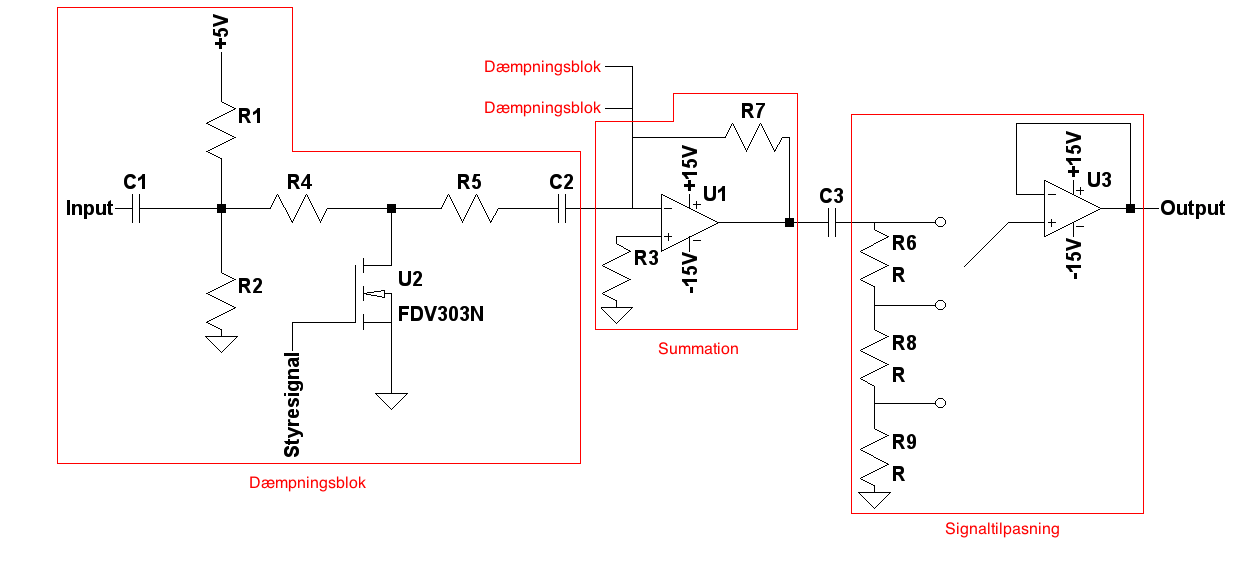
\includegraphics[width=\textwidth]{../rapport/teknisk/indgangsvaelger/signal-taend-sluk.png}
\label{fig:indgangsvaelger-overordnet}
\end{figure}
\end{frame}

\begin{frame}{Indgangsvælger - Styring}

\begin{figure}[h]
\centering
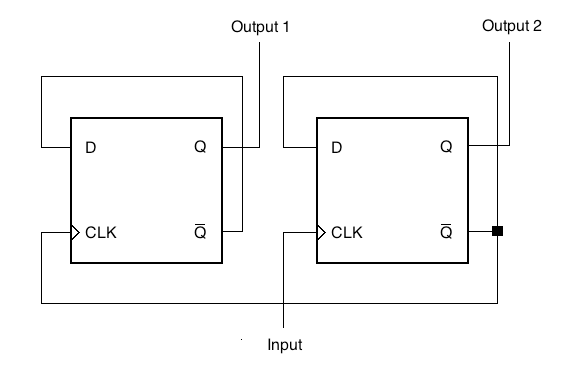
\includegraphics[scale=0.4]{../rapport/teknisk/indgangsvaelger/flipflop.png}
\label{fig:indgangsvaelger-flipflop}
\end{figure}
\end{frame}

\begin{frame}{Indgangsvælger - Simulering}
\begin{figure}[h]
\centering
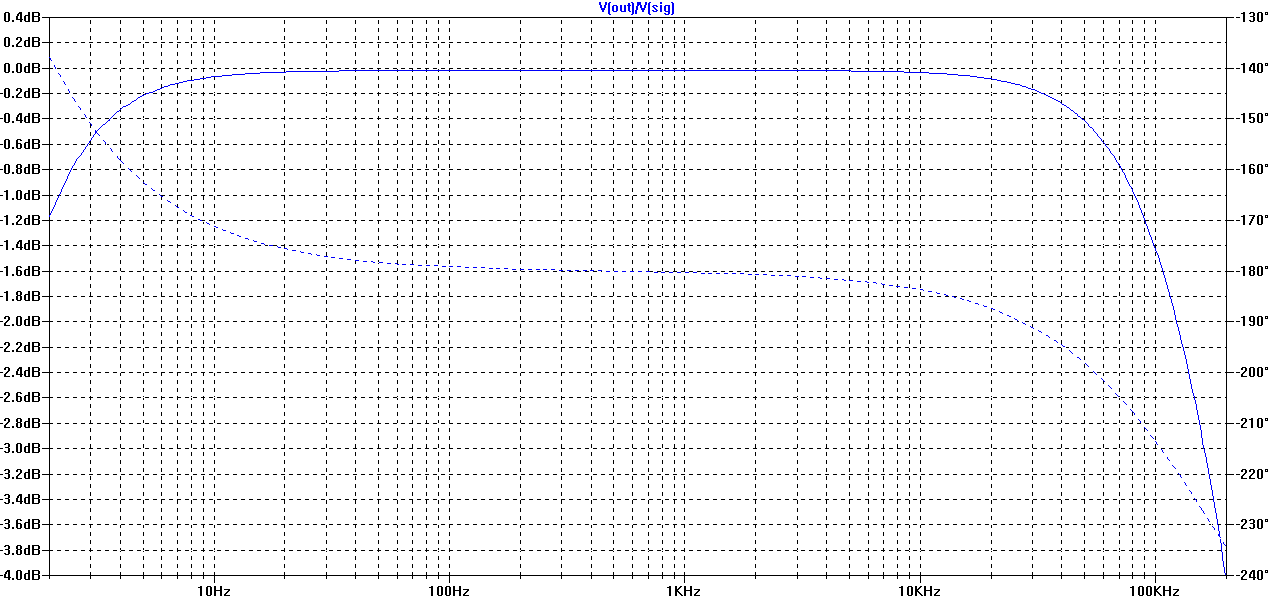
\includegraphics[width=\textwidth]{../rapport/teknisk/indgangsvaelger/simulering/frekvenskarakteristik.png}
\label{indgangsvaelger_frekvenskarakteristik}
\end{figure}
\end{frame}

\begin{frame}{Indgangsvælger - Måling}
\begin{figure}[h]
\centering
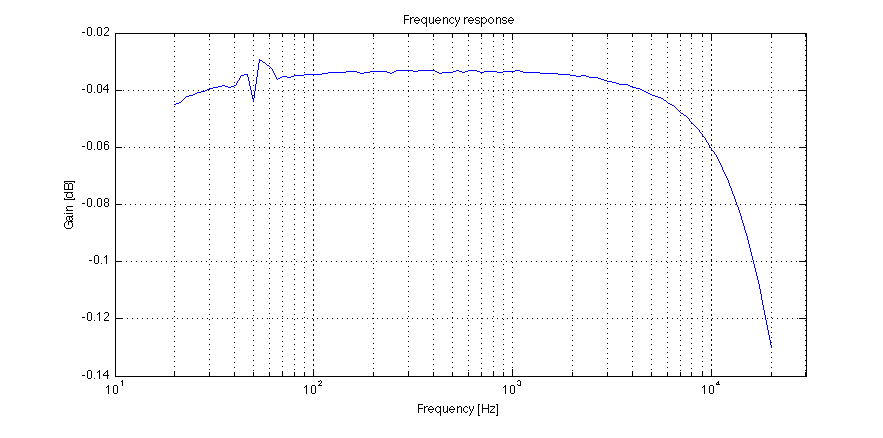
\includegraphics[width=\textwidth]{../rapport/maalerapporter/indgangsvaelger/Indgangsvlger-mic-200mv-frek.png}
\label{fig:indacc:frek200mv}
\end{figure}
\end{frame}

\begin{frame}{Indgangsvælger - Måling}
\begin{figure}[h]
\centering
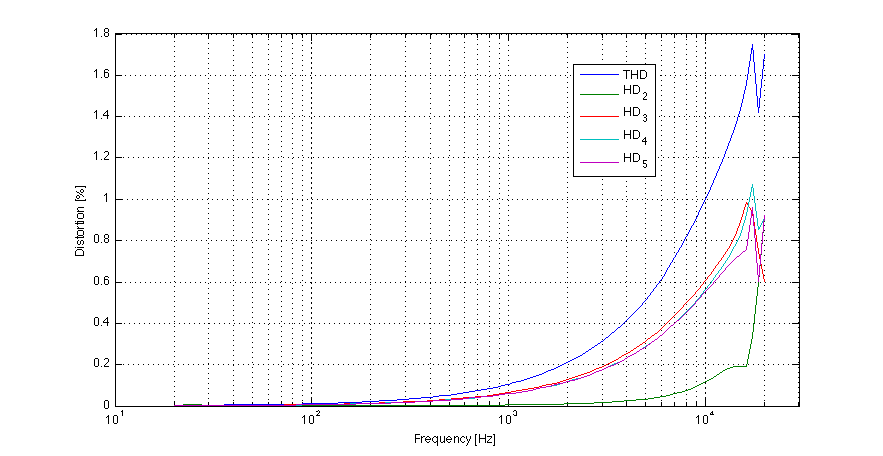
\includegraphics[width=\textwidth]{../rapport/maalerapporter/indgangsvaelger/Indgangsvlger-mic-2v-thd.png}
\label{fig:accind:thd2v}
\end{figure}
\end{frame}


\begin{frame}{Indgangsvælger - Accepttest}
\scriptsize{
\begin{table}[h]
\centering
\begin{tabular}{l|r|r}
\hline\hline
Område & Krav & Status \\
\hline\hline
Antal trin i & 4 & \checkmark \\
indgangsvælgeren & \\[4pt]
Indgangsimpedans & \> 22 k\ohm & \checkmark \\[4pt]
Frekvensgang & \< 0,375 dB ved 20 Hz - 20 kHz, ref. 1 kHz & \checkmark \\
& \< 0,75 dB fra 20 Hz til 63 Hz & \checkmark\\
& \< 0,75 dB fra 12,5 kHz til 20 kHz & \checkmark\\[4pt]
Dæmpning af slukket & \> 50 dB ved 1 kHz & \checkmark \\
indgangssignal & \\
\hline\hline
\end{tabular}
\label{tab:krav_indgangsvaelger}
\end{table}
}
\end{frame}